%%%% Paramétrage du TD %%%%
\def\xxnumchapitre{Chapitre 2 \vspace{.2cm}}
\def\xxchapitre{\hspace{.12cm} Révisions SLCI}

\def\xxcompetences{%
\textsl{%
\textbf{Savoirs et compétences :}\\
\vspace{-.4cm}
\begin{itemize}[label=\ding{112},font=\color{bleuxp}] 
\item .
%\item \textit{Mod3.C2 : } pôles dominants et réduction de l’ordre du modèle : principe, justification
\end{itemize}
}}

\def\xxfigures{

\includegraphics[width=.9\linewidth]{fig_00}
%\textit{}
}%figues de la page de garde

\def\xxtitreexo{Tour en fosse utilisé pour le reprofilage des roues ferroviaires -- Asservissement du porte-outil }
\def\xxsourceexo{\hspace{.2cm} \footnotesize{Concours Centrale Supelec -- PSI 2018}}

\def\xxactivite{{Colle 03} \ifprof  -- Corrigé \else \fi}


\input{\repRel/Style/pagegarde_TD}


\setlength{\columnseprule}{.1pt}

\pagestyle{fancy}
\thispagestyle{plain}

\vspace{5cm}

\def\columnseprulecolor{\color{bleuxp}}
\setlength{\columnseprule}{0.4pt} 
\setcounter{numques}{0}
%%%%%%%%%%%%%%%%%%%%%%%

\ifprof
\else
\begin{multicols}{2}
\fi

\subsection*{Modélisation du mouvement pour la commande}
\begin{obj}
Modéliser le comportement dynamique de l’outil et du porte-outil, puis étudier une commande en
position $z_1(t)$ comprenant un correcteur proportionnel.
\end{obj}

Le système composé de l’outil et du porte-outil est modélisé sur la \autoref{fig_10}. Le porte-outil, de masse $m_1 = \SI{5522}{kg}$,
est considéré indéformable et en liaison glissière de direction $\vect{z_0}$ avec le bâti. Une chaîne de motorisation électrique
permet de déplacer le porte-outil et une structure de commande associée permet d’asservir la position
$z_1(t)$ par rapport à une position de référence. La chaîne de motorisation exerce une force motrice $\vect{f}_m(t) =f_m(t)\vect{z_0}$
sur le porte-outil.

La cahier des charges est donné sur la figure suivante.



\begin{figure}[H]
\centering
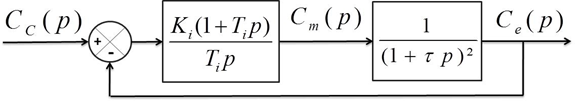
\includegraphics[width=\linewidth]{fig_08}
\caption{Diagramme des exigences de la chaîne d'asservissement \label{fig_08}}
\end{figure}




Les positions du porte-outil et du point $C$  par rapport à leur position de référence sont respectivement paramétrées
par $z_1(t)\vect{z_0}$ et $z_2(t)\vect{z_0}$, avec $z_1(t)\vect{z_0}$ et $z_2(t)\vect{z_0}$ des grandeurs algébriques ( \autoref{fig_10}). Les conditions initiales
sont toujours supposées nulles.


Le théorème de la résultante dynamique appliqué au porte-outil puis à l’outil permet d’obtenir les deux relations
suivantes :
$$
\begin{array}{l}
m_1\ddot{z}_1(t)+\lambda\dot{z}_1(t)+Kz_1(t) = \lambda\dot{z}_2(t)+Kz_2(t)+f_m(t) \\
m_2\ddot{z}_2(t)+\lambda\dot{z}_2(t)+Kz_2(t) = \lambda\dot{z}_1(t)+Kz_1(t)+f_c(t) \\
\end{array} $$
Le modèle correspondant est représenté par le schéma bloc de la  \autoref{fig_11}.

\begin{figure}[H]
\centering
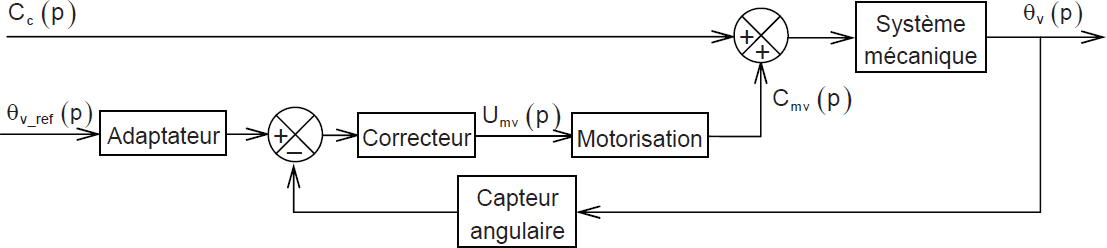
\includegraphics[width=.7\linewidth]{fig_10}
\caption{Modèle de déformation de l'outil avec le porte-outil piloté \label{fig_10}}
\end{figure}

\begin{figure}[H]
\centering
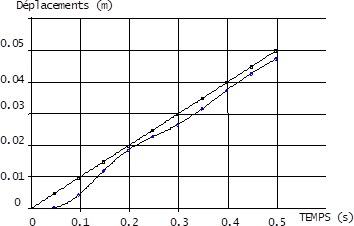
\includegraphics[width=.9\linewidth]{fig_11}
\caption{Modèle de l'outil et du porte-outil \label{fig_11}}
\end{figure}


\question{Exprimer les fonctions $H_1(p)$, $H_2(p)$, $H_3(p)$ et $H_4(p)$ en fonction de $K$, $\lambda$, $m_1$ et $m_2$.}

Le modèle de la  \autoref{fig_11} est réduit au modèle équivalent de la figure \autoref{fig_12}.


\begin{figure}[H]
\centering
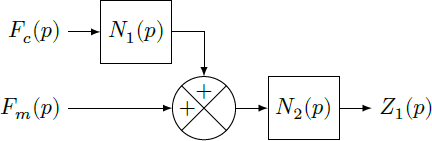
\includegraphics[width=.7\linewidth]{fig_12}
\caption{Modèle équivalent \label{fig_12}}
\end{figure}


\question{Exprimer $N_1(p)$ et $N_2(p)$ en fonction de $H_1(p)$, $H_2(p)$, $H_3(p)$ et $H_4(p)$.}

\question{Montrer que $N_2(p)$ peut s’écrire sous la forme $N_2(p) = A\dfrac{p^2+2\xi_1\omega_1 p + \omega_1^2}{p^2\left( p^2+2\xi_2\omega_2p + \omega_2^2\right)}$. Exprimer $\xi_1$, $\xi_2$, $\omega_1$, $\omega_2$ et $A$ en fonction de $m_1$n $m_2$, $\lambda$ et $K$.}

Le diagramme de Bode associé à la fonction de transfert $N_2(p)$ est représenté ci-après.


\begin{figure}[H]
\centering
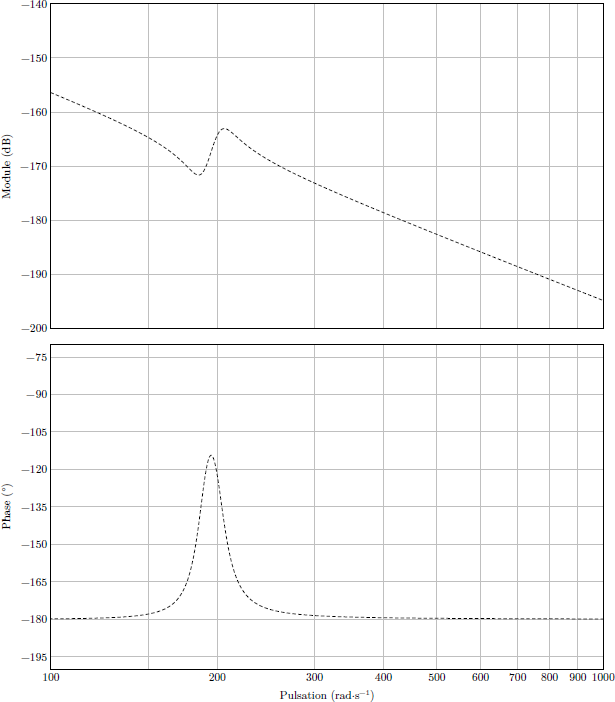
\includegraphics[width=\linewidth]{fig_dr}
%\caption{Modèle équivalent}
\end{figure}


\question{Compléter ce diagramme par les tracés asymptotiques en module et en phase, et conclure sur la
cohérence du diagramme donné.}

\question{Au regard des valeurs numériques, montrer que la fonction de transfert $N_2(p)$ peut être approchée
par la fonction $N_{2 \text{app}}(p)=\dfrac{A}{p^2}$. En utilisant une couleur différente, tracer le diagramme de Bode associé à la
fonction de transfert $N_{2 \text{app}}(p)$ sur le document réponse et conclure sur la validité de ce modèle approché.}

Le modèle approché ($N_{2 \text{app}}(p)$) est retenu pour la suite de l’étude. Le schéma bloc modélisant la régulation de
la position $z_1(t)$ est donné en figure \autoref{fig_13}, en considérant un correcteur proportionnel de gain $K_p$.


\begin{figure}[H]
\centering
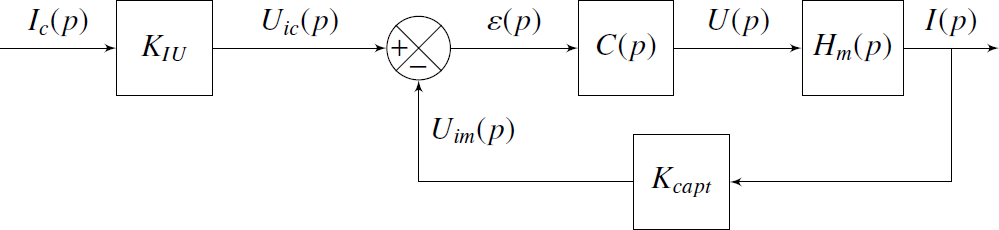
\includegraphics[width=.8\linewidth]{fig_13}
\caption{Modèle de synthèse de la régulation en position $z_1(t)$ du porte-outil \label{fig_13}}
\end{figure}


\question{Justifier qu’une correction proportionnelle ne permet pas de respecter l’ensemble des critères du diagramme
des exigences de la \autoref{fig_08}.}


\subsection*{Analyse de l'influence d'un paramètre}

On a d'une part $Q(p) =Q_c (p)-Z_2(p)H_r (p)$. 

D'autre part, la quantité de matière enlevée est donnée par $q(t)=q_c(t)-z_2(t)+z_2\left( t-\tau\right)$ où $\tau$ est la durée nécessaire à la roue pour effectuer
un tour complet. 

D’un point de vue numérique, $K_f = 1,5 \times 10^9 \si{N.m^{-2}}$ et $\tau = \SI{1}{s}$. 

\question{Déterminer $H_r(p)$ en fonction de $\tau$.}

Le schéma-blocs retenu est le suivant. 

\begin{figure}[H]
\centering
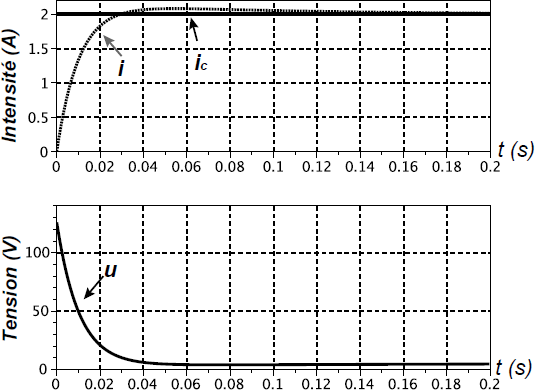
\includegraphics[width=.65\linewidth]{fig_16}
\caption{Modèle équivalent de la chaîne d'asservissement complète\label{fig_16}}
\end{figure}


La \autoref{fig_17} représente le diagramme de Bode de la fonction de transfert en boucle ouverte du système modélisé
\autoref{fig_16}, avec $b=\dfrac{5\times 10^{-2}}{\pi} \si{mm.rad^{-1}}$

\begin{figure}[H]
\centering
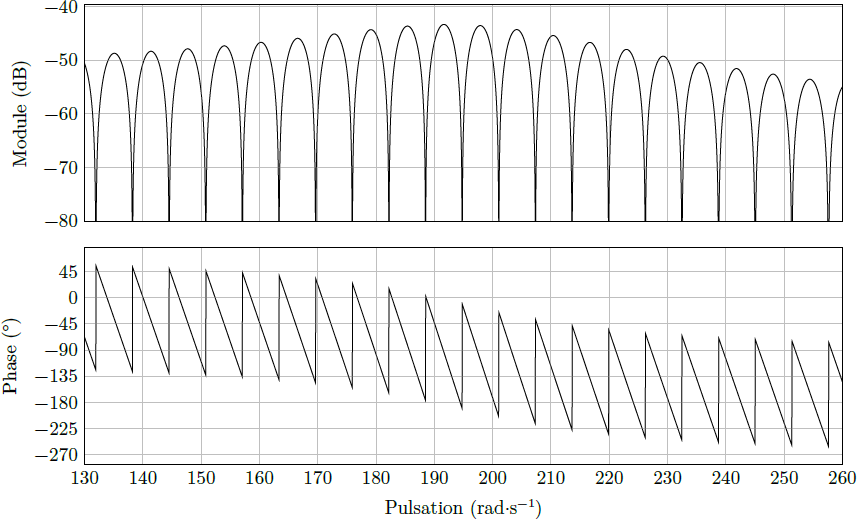
\includegraphics[width=\linewidth]{fig_17}
\caption{Diagramme de Bode de la boucle ouverte du schéma-blocs\label{fig_17}}
\end{figure}


Les « zéros de transmission » d’une fonction de transfert $H(p)$ correspondent aux pulsations $\omega$ pour lesquelles
$H\left(j \omega\right)$ est nul.

\question{Préciser l’expression de la fonction de transfert en boucle ouverte de la figure 16 puis vérifier la
cohérence du diagramme de Bode de la\autoref{fig_17}  en analysant les « zéros de transmission ».}

\question{Déterminer un ordre de grandeur du paramètre $b$ permettant de conserver la stabilité du système en
boucle fermée. Conclure sur la compatibilité de cette valeur maximale avec un bon amortissement de l’asservissement.}

\ifprof
\else
\end{multicols}
\fi

